\documentclass[12pt,a4]{article} %[font size, tamano de hoja]{Tipo de documento}

\usepackage[left=1.8cm,right=1.8cm,top=32mm,columnsep=20pt]{geometry}

\usepackage[utf8]{inputenc} %Formato de codificación
\usepackage[spanish, es-tabla, es-nodecimaldot]{babel}
\usepackage{amsmath} %paquete para escribir ecuaciones matemáticas
\usepackage{float} %Para posicionar figuras
\usepackage{graphicx} %Para poder poner figuras
\usepackage{hyperref} %Permite usar hipervínculos 
\usepackage{multicol} %Para hacer doble columna
\usepackage[sorting=none]{biblatex} %Imports biblatex package. To cite use \cite{reference_label}
\addbibresource{main.bib} %Import the bibliography file



\title{Métodos Numéricos y Optimización\\

 Trabajo práctico N$^{\circ}$1\\
\vspace{20mm}

 Interpolación y búsqueda de raíces
}

\author{Valentino Arbelaiz y Alejo Zimmermann\\ [2mm] %\\ para nueva línea
\small Universidad de San Andres, Buenos Aires, Argentina}
\date{1er Semestre 2024}
% Tamanos de letra: 
% \tiny	
% \scriptsize
% \footnotesize
% \small	
% \normalsize	
% \large	
% \Large	
% \LARGE	
% \huge	
% \Huge


%Todo lo que está antes de begin{document} es el preámbulo
\begin{document}
\vspace{1cm} % Ajusta la distancia vertical entre la fecha y la imagen



\maketitle
% \begin{center}
% \includegraphics[width=5cm]{logoUdesa.png} % Ajusta la ruta y el tamaño de la imagen
% \end{center}


\begin{abstract}
    Este trabajo estudia el efecto de la distribución de puntos de interpolación en esquemas numéricos de aproximación de funciones uni y bidimensionales, proponiendo una regla para puntos no equiespaciados. Además, se aborda la reconstrucción de trayectorias de vehículos autónomos a partir de mediciones de posición mediante interpolación, determinando el punto de intersección entre dos trayectorias.
\vspace{2mm}
\end{abstract}

\begin{multicols}{2}
\raggedcolumns

\section{Introducción}
En este trabajo se abordan dos problemas generales de los métodos numéricos. Aproximación de funciones y reconstrucción de trayectorias a partir de puntos en un plano.

En la primera parte, se estudiará el efecto que tiene la distribución de los puntos de interpolación en el desempeño de distintos esquemas de interpolación polinómica y spline. Se analizarán funciones unidimensionales y bidimensionales, utilizando inicialmente puntos de colocación equiespaciados. Luego, utilizando los polinomios de Chebyshev para seleccionar puntos de interpolación no equiespaciados y se compararon los resultados obtenidos con los de la distribución equiespaciada estándar.

En la segunda parte, se aplicarán técnicas de interpolación para reconstruir trayectorias de vehículos autónomos a partir de mediciones discretas de su posición. Utilizando un conjunto de datos de posiciones, se recuperará la trayectoria de un primer vehículo y se contrastará con la trayectoria real provista. Adicionalmente, se abordará la determinación del punto de intersección entre la trayectoria reconstruida y la de un segundo vehículo a partir de un conjunto más reducido de mediciones de posición.



\section{Métodos}

\textit{A lo largo del trabajo utilizamos los siguientes métodos. }

\subsection{Interpolación}

En la primer seccion de la investigación se estudiaron diversas maneras de interpolación en dos funciones distintas.
\subsubsection{Interpolación de Lagrange}
La Interpolación de Lagrange es un método para encontrar un polinomio que pase por un conjunto dado de puntos. La fórmula para el polinomio interpolante de Lagrange es:

\begin{equation}
    L(x) = \sum_{i=0}^{n} y_i \prod_{j=0, j\neq i}^{n} \frac{x - x_j}{x_i - x_j}
    \label{lagrange}
\end{equation}

Donde $(x_i, y_i)$ son los puntos dados. Este método es útil cuando se tienen pocos puntos y se desea obtener un polinomio que los interpole. Sin embargo, para un gran número de puntos, el polinomio resultante puede oscilar significativamente.
\subsubsection{Interpolación con splines}
El método de interpolación con splines está basado en la interpolación a trozos (piecewise-polynomial interpolation) lo cual consiste en dividir el intervalo principal en subintervalos y realizar una interpolación independiente en cada uno de ellos. La más sencilla es la interpolación lineal a trozos, generando una recta entre cada uno de los nodos. También existe la cuadrática generando funciones cuadráticas en cada subintervalo. Dentro de todos los métodos que existen de interpolación a trozos, en este trabajo se utilizaron los splines cúbicos.

\begin{equation}
    S(x) = a_i + b_i(x - x_i) + c_i(x - x_i)^2 + d_i(x - x_i)^3
    \label{spline cubico}
\end{equation}

Donde $(x_i, y_i)$ son los puntos dados y $a_i$, $b_i$, $c_i$, $d_i$ son los coeficientes del polinomio para el i-ésimo subconjunto. Este método es útil cuando se tienen muchos puntos y se desea obtener una función que los interpole de manera suave, evitando las oscilaciones que pueden ocurrir con la Interpolación de Lagrange.

\subsubsection{Calculo del error}
En el trabajo contamos con la ventaja de conocer la función sobre la cual estamos interpolando, por lo tanto, podemos comparar el error de la siguiente forma: calcular los valores de la función real $f(x)$ en los puntos y compararlos con los valores interpolados $\hat{f}(x_j)$ obtenidos mediante los métodos de interpolación estudiados de este modo:

\begin{equation}
    \int_{a}^{b} |f(x) - \hat{f}(x_j) | \,  dx
\end{equation}

Donde $(a, b)$ es el intervalo de $\hat{f}(x_j)$


\subsection{Raíces de Chebyshev}
Los puntos de Chebyshev son un conjunto de puntos utilizados en los métodos numéricos principalmente en la aproximación de funciones. Estos puntos son el conjunto de soluciones de la función de Chebyshev \eqref{Raices Chebyshev}. Pueden generar un impacto en la precisión de las aproximaciones de funciones como durante la interpolación. 
\begin{equation}
    x_{k} = \frac{(a+b)}{2} + \frac{(b-a)}{2} \cos \left( \frac{2k+1}{2n} \pi \right),   
    \label{Raices Chebyshev}
\end{equation}
Con $ k = 0, \ldots, n-1.$ y $n$ es la cantidad de nodos en el intervalo $[a,b]$

\subsection{Búsqueda de raíces}
En la segunda parte, se determinaron las coordenadas en las cuales se cruzan las trayectorias.
\subsubsection{Newton-Raphson}
El método de Newton-Raphson, es un procedimiento iterativo para encontrar aproximaciones numéricas de las raíces de una función $f(x)$. Este método se basa en la construcción de una sucesión de valores que convergen a una raíz de la función, partiendo de una estimación inicial $x_0$.

En cada iteración $n$, se calcula la pendiente de la recta tangente a la función $f(x)$ en el punto $x_n$, es decir, $f'(x_n)$. Luego, se determina la intersección de esta recta tangente con el eje de las abscisas, que brinda una mejor aproximación $x_{n+1}$ a la raíz de la función. Este proceso se repite hasta alcanzar un nivel de precisión deseado o hasta que se cumpla algún criterio de convergencia.

La fórmula de iteración del método de Newton-Raphson viene dada por:

\begin{equation}
    x_{n+1} = x_n - \frac{f(x_n)}{f'(x_n)}
\end{equation}

donde $x_n$ es la aproximación en la n-ésima iteración, $f(x_n)$ es el valor de la función en $x_n$, y $f'(x_n)$ es la derivada de la función en $x_n$. 
\subsubsection{Método de Newton-Raphson}

El método de Newton-Raphson, también conocido como el método de Newton, es un procedimiento iterativo para encontrar aproximaciones numéricas de las raíces de una función $f(x)$. Este método se basa en la construcción de una sucesión de valores que convergen a una raíz de la función, partiendo de una estimación inicial $x_0$.

En cada iteración $n$, se calcula la pendiente de la recta tangente a la función $f(x)$ en el punto $x_n$, es decir, $f'(x_n)$. Luego, se determina la intersección de esta recta tangente con el eje de las abscisas, que brinda una mejor aproximación $x_{n+1}$ a la raíz de la función. Este proceso se repite hasta alcanzar un nivel de precisión deseado o hasta que se cumpla algún criterio de convergencia.

La fórmula iterativa del método de Newton-Raphson viene dada por:

\begin{equation}
x_{n+1} = x_n - \frac{f(x_n)}{f'(x_n)}
\label{eq:newton_raphson}
\end{equation}

Donde $f(x_n)$ es el valor de la función evaluada en $x_n$, y $f'(x_n)$ es la derivada de la función evaluada en $x_n$.

Este método tiene una convergencia rápida, con un orden de convergencia cuadrático, siempre que la estimación inicial $x_0$ se encuentre lo suficientemente cerca de la raíz y que la función cumpla ciertas condiciones de derivabilidad en un entorno de la raíz.

El método también se puede extender a sistemas de ecuaciones no lineales en mayores dimensiones. En este caso, la fórmula iterativa involucra el cálculo del jacobiano de la función en lugar de su derivada.


\section{Implementación}

Los métodos previamente presentados se aplicaron a lo largo del proyecto. En la primera sección, se investigó el comportamiento de la interpolación de dos funciones analizadas por separado

La primer función $f_a(x)$ fue definida mediante la librería NumPy de Python:
\begin{equation}
    f_a (x) = 0.3 ^{|x|}  \cdot \sin(4x) - \tanh(2x) + 2
    \label{$f_a(x)$}
\end{equation}
\hspace{6mm}con $x \in [-4,4]$
\vspace{3 mm}

La función $f_b(x)$ es la siguiente:
\begin{multline*}  
    f_b(x) = 0.75exp\left(-\frac{(10x_1-2)^2}{4}-\frac{(9x_2-2)^2}{4}\right)\\
+0.65exp\left(-\frac{(9x_1+1)^2}{9}-\frac{(10x_2+1)^2}{2}\right)\\
+0.55exp\left(-\frac{(9x_1-6)^2}{4}-\frac{(9x_2-2)^3}{4}\right)\\
-0.01exp\left(-\frac{(9x_1-7)^2}{4}-\frac{(9x_2-3)^2}{4}\right)
\label{$f_a(x)$}
\end{multline*}
\hspace{6mm}con $x\in[-1,1]$


Los intervalos fueron divididos en nodos equiespaciados y fueron almacenados en un arreglo de NumPy. Se interpolan las funciones utilizando la librería SciPy, aplicando los métodos mencionados anteriormente.
Se estudió el desarrollo de las funciones a medida que se aumentaba la cantidad de nodos.
Para la primera función calculamos el error de la interpolación a través de las integrales, comparando cómo varía el error según el método y la cantidad de nodos. También comparamos los errores con puntos no equiespaciados utilizando los nodos de Chebyshev.

En la segunda parte, se utilizaron splines cúbicos para reconstruir la trayectoria de un vehículo en distintos instantes de tiempo. Luego, se comparó esta misma trayectoria con la de otro vehículo, con el fin de determinar en que coordenadas los vehículos atraviesan sus trayectorias. Para calcular la intersección se utilizo el método Newton-Rhapson con cálculo multivariable. 

\section{Resultados y análisis}

\subsection{Interpolación de $f_a(x)$ }
Se interpoló la función de multiples maneras. La función fue definida con 1000 puntos con el motivo de conseguir una representación de la función mas suave. Para el método de interpolación de Lagrange \eqref{lagrange} se dividió el intervalo $[-4,4]$ en 5 y en 8 puntos equiespaciados para analizar el comportamiento de la función con diferentes parametros. 
\begin{figure}[H]
    \centering
    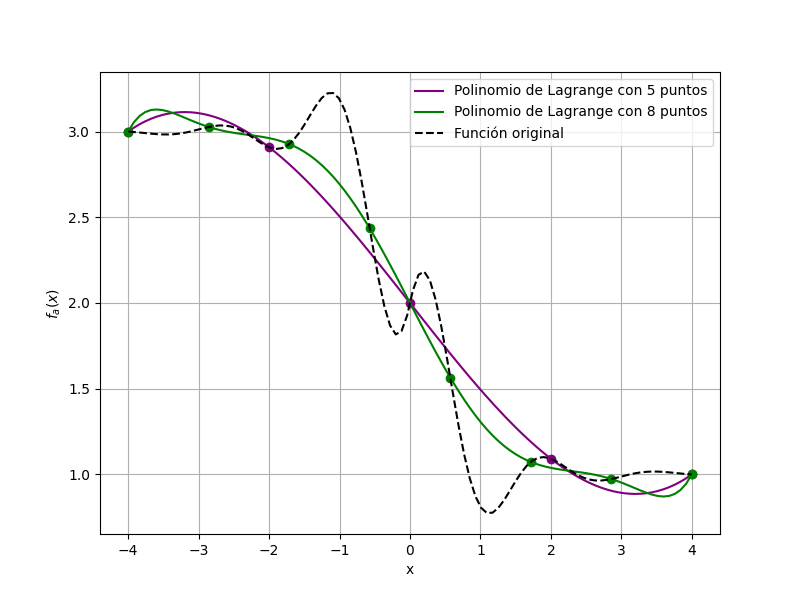
\includegraphics[width=0.5\textwidth]{lagrange.png}
    \caption{Comparación de la interpolación de Lagrange de $f_a(x)$ con distintos nodos equiespaciados.}
    \label{fig:Lagrange}
\end{figure}
Por el otro lado, para la interpolación con splines \eqref{spline cubico} se dividió el intervalo en 5 y 12 puntos equiespaciados como muestra la figura \ref{fig:Splines}. 
\begin{figure}[H]
    \centering
    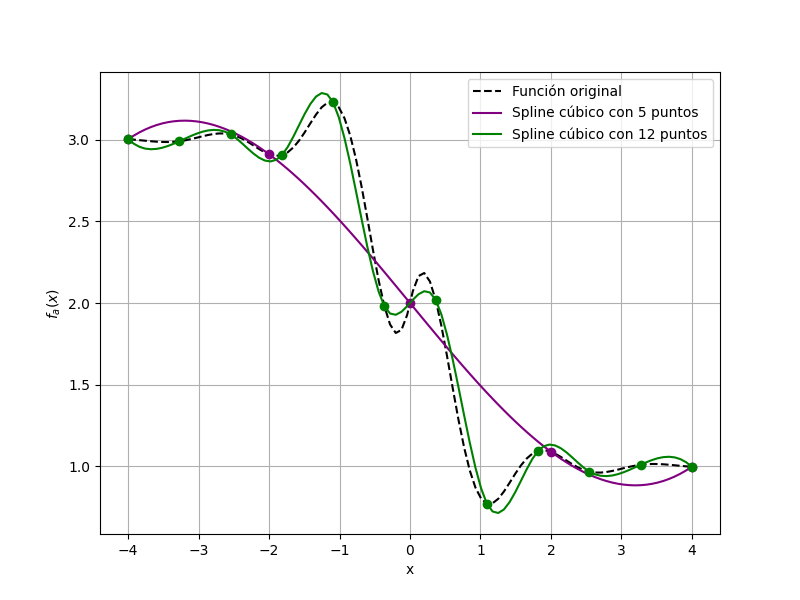
\includegraphics[width=0.5\textwidth]{splines.png}
    \caption{Comparación de la interpolación con splines de $f_a(x)$ con distintos nodos equiespaciados.}
    \label{fig:Splines}
\end{figure}
Se puede apreciar que a mayor cantidad de puntos, la interpolación con splines representa mejor la función a comparación que con el método de Lagrange. Podemos contemplar la evolución del error con el siguiente gráfico:

\begin{figure}[H]
    \centering
    \includegraphics[width=0.5\textwidth]{Lagrange_vs_Splines.png}
    \caption{Comparación de la evolución del error de $f_a(x)$ con el incremento en la cantidad de nodos}
    \label{fig:lagrange_splines_errors}
\end{figure}


\begin{figure}[H]
    \centering
    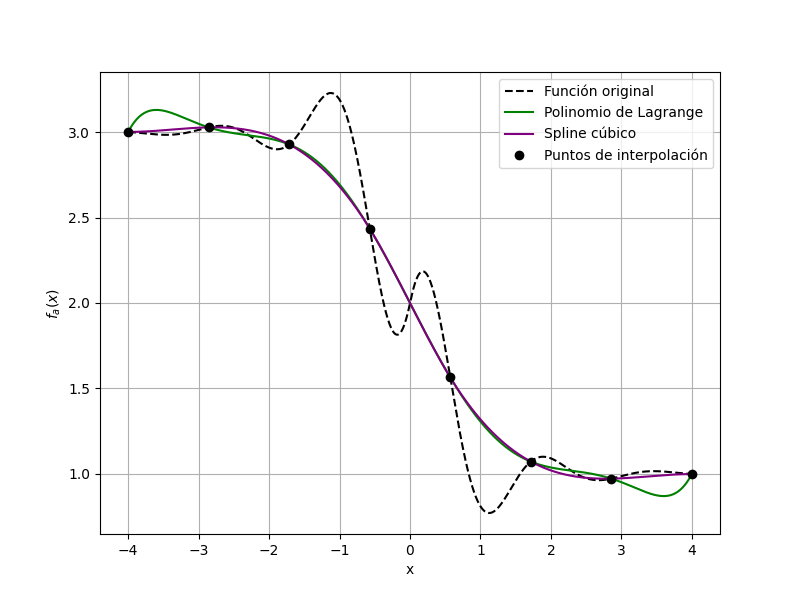
\includegraphics[width=0.55\textwidth]{lagrange_splines_equidistantes.png}
    \caption{Comparación $f_a(x)$ interpolada con Lagrange y splines cúbicos}
    \label{fig:lagrange_splines}
\end{figure}
Se repitió el mismo proceso para puntos no equiespaciados mediante las raíces de Chebyshev \eqref{Raices Chebyshev}. El comportamiento de las funciones con los puntos de Chebyshev generan menos error en los extremos del dominio. 
\begin{figure}[H]
    \centering
    \includegraphics[width=0.55\textwidth]{interpolacion_chebyshev.png}
    \caption{$f_a(x$) interpolado en 12 puntos de Chebyshev}
    \label{fig:cheby points}
\end{figure}
En las figuras \ref{fig:error absoluto equi} y \ref{fig:error absoluto Cheb} se ven los errores absolutos de las diferentes funciones. Estos fueron calculados generando un nuevo polinomio $h(x) = |f_a(x)-interpolacion(f_a(x))|$, por eso las raíces de este nuevo polinomio son en los nodos. 

\begin{figure}[H]
    \centering
    \includegraphics[width=0.55\textwidth]{errores_absolutos_equis.png}
    \caption{Error absoluto de $f_a(x)$ con 12 puntos equiespaciados.}
    \label{fig:error absoluto equi}
\end{figure}

\begin{figure}[H]
    \centering
    \includegraphics[width=0.55\textwidth]{errores_absolutos_chebyshev.png}
    \caption{Error absoluto de $f_a(x)$ con 12 puntos de Chebyshev.}
    \label{fig:error absoluto Cheb}
\end{figure}

La figura \ref{fig:error absoluto equi} demuestra un error absoluto mayor en los extremos que la figura \ref{fig:error absoluto Cheb}. 

\begin{figure}[H]
    \centering
    \includegraphics[width=0.55\textwidth]{funcion_b.png}
    \caption{Función $f_b(x)$}
    \label{fig:funcion b}
\end{figure} 
La función $f_b(x_1,x_2)$ se analizó en $R^2$ usando griddata para interpolarla \ref{fig:inter b equi} y matplotlib para graficarla. La función se graficó con una base de $100 x 100$ puntos generando una alta presición al ser graficada. 
\begin{figure}[H]
    \centering
    \includegraphics[width=0.55\textwidth]{interpolacion_b.png}
    \caption{Interpolación de la función $f_b(x)$ puntos equiespaciados}
    \label{fig:inter b equi}
\end{figure}

\begin{figure}[H]
    \centering
    \includegraphics[width=0.55\textwidth]{interpolacion_chebyshev_b.png}
    \caption{Interpolación de la función $f_b(x)$ con puntos de Chebyshev}
    \label{fig:enter-label}
\end{figure}
\subsubsection{Búsqueda de raíces y reconstrucción de trayectorias}



Escrubi aca valen \ref{fig:lagrange_splines}
\section{Conclusión}


En la primera parte del trabajo, se realizaron interpolaciones de la función $f_a(x)$ utilizando diferentes métodos, como Lagrange y splines cúbicos. Se observó que a medida que se aumentaba la cantidad de nodos, la interpolación con splines cúbicos representaba mejor la función en comparación con el método de Lagrange. Además, se encontró que la utilización de puntos no equiespaciados, como las raíces de Chebyshev, generaba menos error en los extremos del dominio.

Estos resultados demuestran la importancia de elegir el método de interpolación adecuado y la distribución de los nodos para obtener una representación precisa de la función. En la siguiente parte del trabajo, se abordará la búsqueda de raíces y la reconstrucción de trayectorias utilizando los conceptos de interpolación estudiados en esta sección.
